\section{Stand der Technik}
W\"{a}hrend der Einarbeitungszeit sind wir durch Literaturrecherche auf einige Dissertationen, Abschlussarbeiten und Richtlinien aufmerksam geworden, welche vergleichbare Versuchsaufbauten beinhalten, weche haupts\"{a}chlich zur Kalibrierung von Partikelmessger\"{a}ten dienen.

Die Masterarbeit \ref{xyz} hatte das Ziel das Ansprechverhalten einer Constant Volume Sampling (CVS) Anlage zu optimieren. Der daf\"{u}r verwendete Versuchsaufbau ist in Abbildung \ref{fig:aufbau_graz} abgebildet. Das hierf\"{u}r verwendete Aerosol wurde aus den Abgasen eines Versuchsfahzeugs entnommen und zusammen mit Verd\"{u}nnungsluft in einen CVS Tunnel geleitet, in welchem sich ein Partikelmesssystem befindet. Die Partikeltestsignale wurden hierbei mit Hilfe eines Umschalters erzeugt, bei dem zwischen einem Aerosolstrom und Luftstrom geschaltet werden kann (Abbildung \ref{fig:umschalter_graz}). Diese M\"{o}glichkeit der Generierung eines Partikeltestsignals wurde in die Erarbeitung von unseren Konzepten miteinbezogen. Zudem k\"{o}nnte der CVS Tunnel f\"{u}r nachfolgende Arbeiten, welche sich ausschlie{\ss}lich mit den Str\"{o}mungen der Aerosole besch\"{a}ftigen w\"{u}rde, von Interesse sein.

\begin{figure}[H]
	\myfloatalign
	{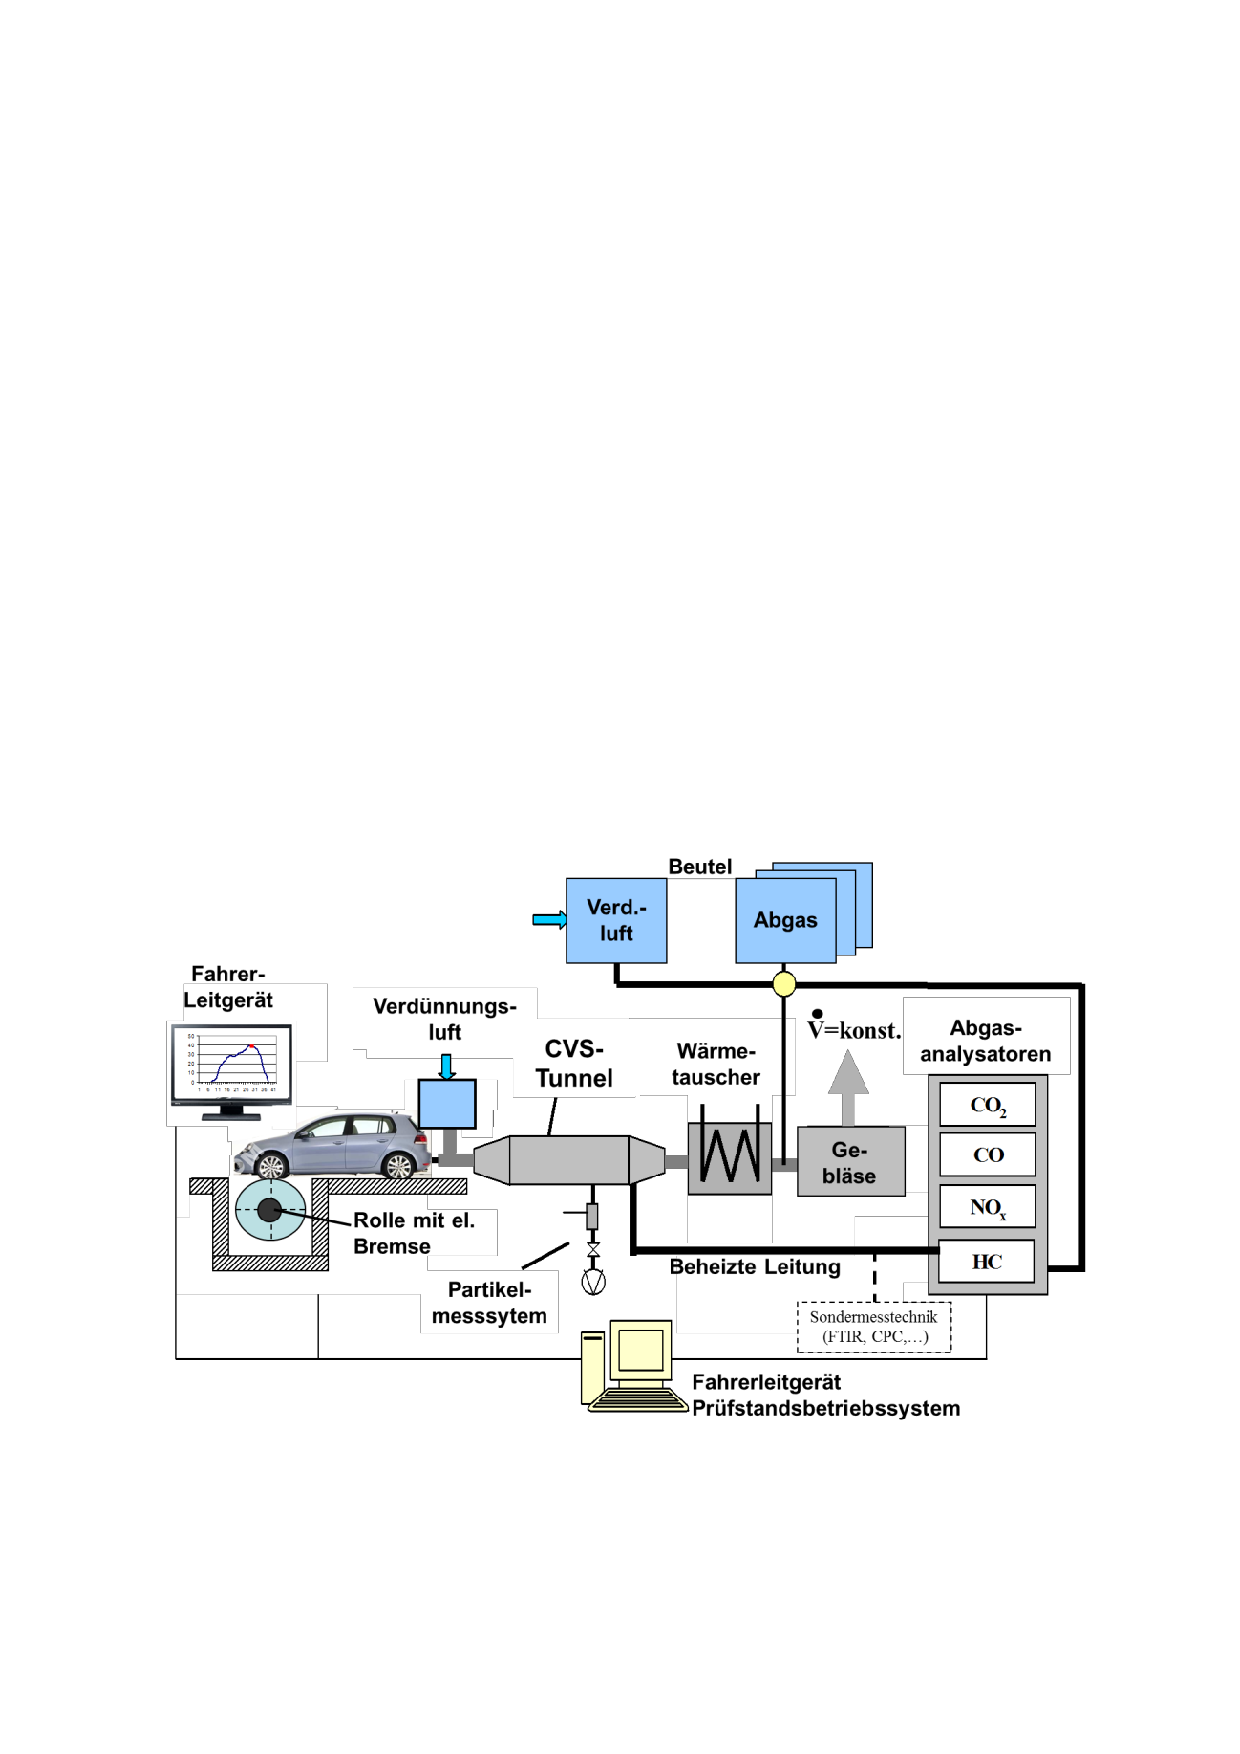
\includegraphics[width=.9\linewidth]{gfx/related/graz_versuch.pdf}} \quad
	\caption[Versuchsaufbau der TU Graz (Quelle: \cite{tu_graz}, S.2)]
	{Versuchsaufbau der TU Graz (Quelle: \cite{tu_graz}, S.2)}
	\label{fig:aufbau_graz}
\end{figure}
\begin{figure}[H]
	\myfloatalign
	{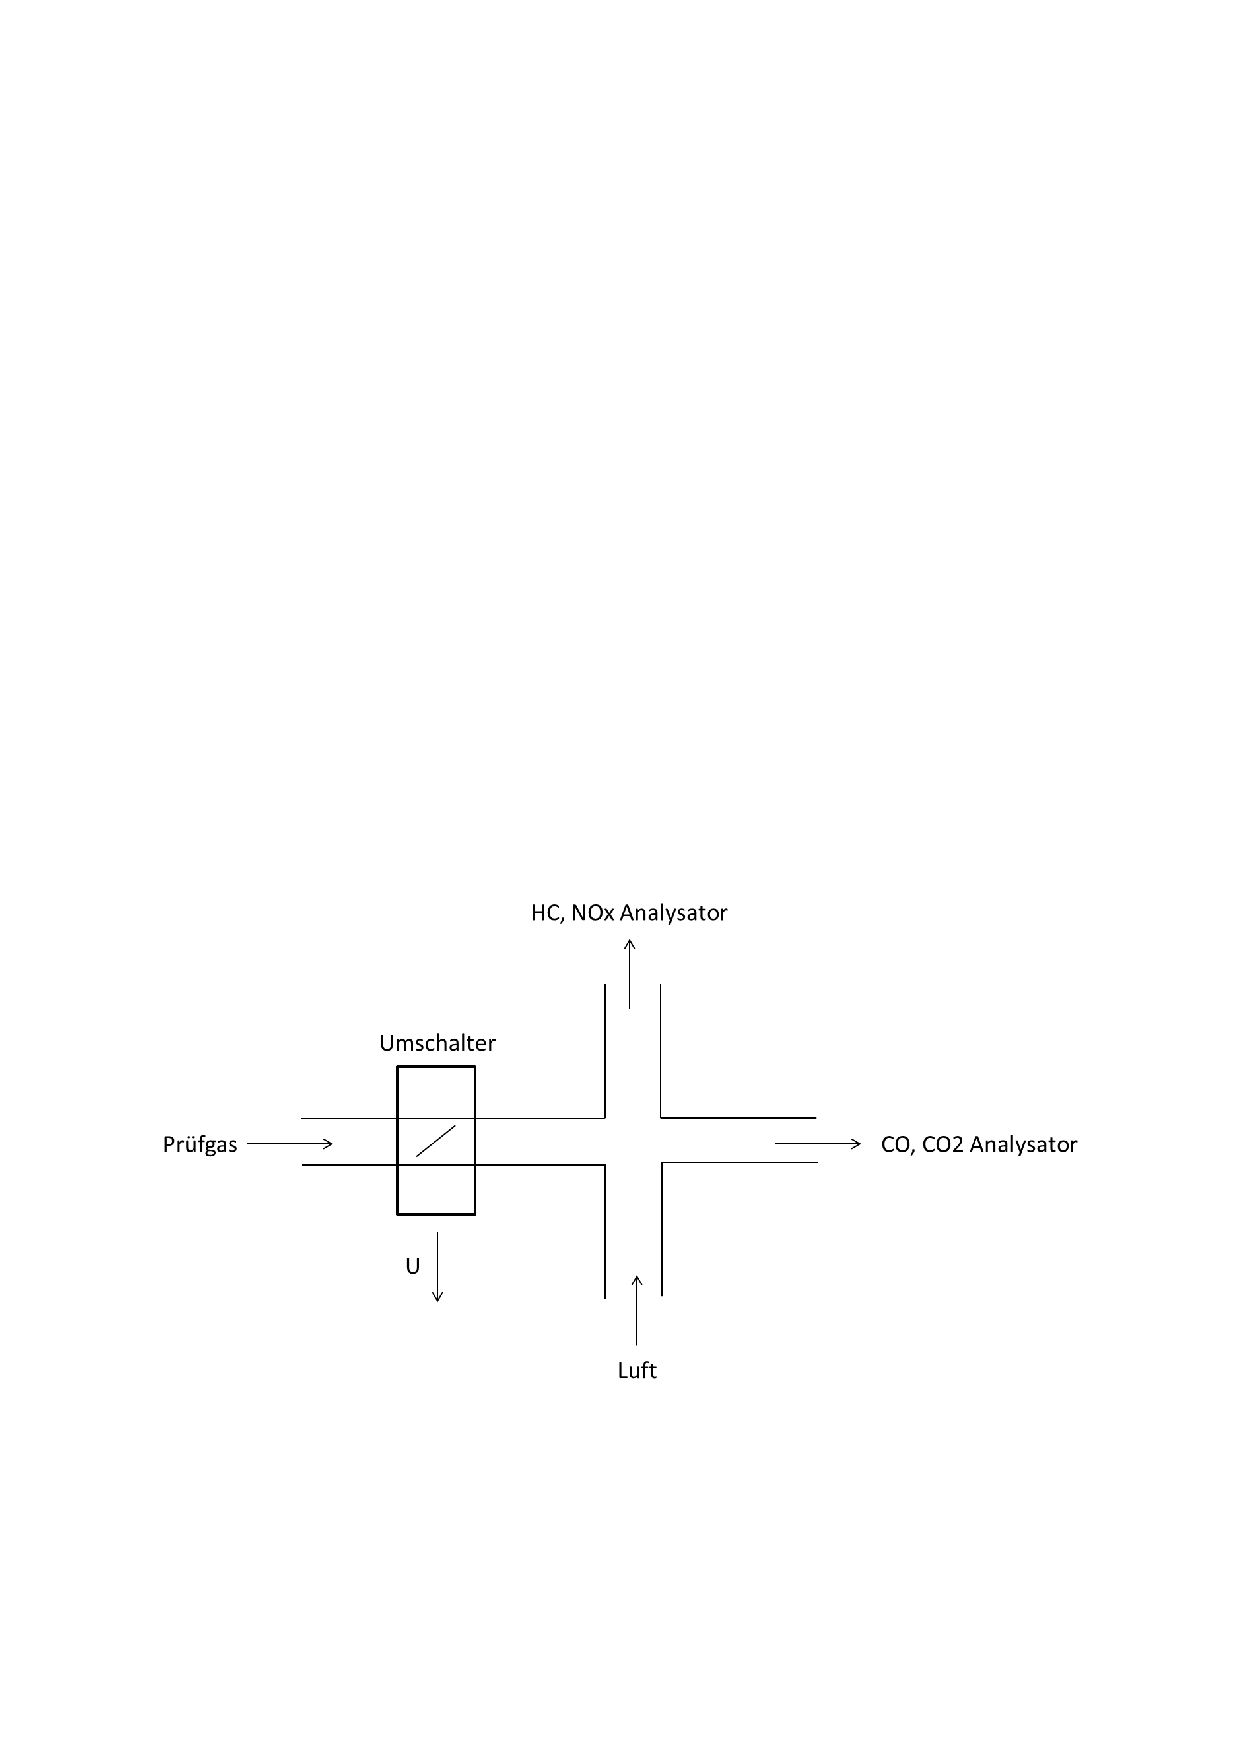
\includegraphics[width=.9\linewidth]{gfx/related/graz_ventil.pdf}} \quad
	\caption[Umschalter vom Versuchsaufbau der TU Graz (Quelle: \cite{tu_graz}, S.12)]
	{Umschalter vom Versuchsaufbau der TU Graz (Quelle: \cite{tu_graz}, S.12)}
	\label{fig:umschalter_graz}
\end{figure}

In \cite{kerze} wird die chemische Zusammensetzung von Kerzenrauch untersucht. Diese Arbeit beinhaltet zwei Punkte, welche f\"{u}r unser Projekt von Interess waren. Zum einen zeigt die Arbeit, dass sich Kerzenrauch unter bestimmten Bedinungen als Pr\"{u}faeorosol eignet. Zum anderen stellt der verwendete Versuchsaufbau (Abbildung \ref{fig:kerze_exp}) eine M\"{o}glichkeit dar, wie eine solche Aerosolprobe zu einem Partikelmessger\"{a}t gef\"{u}hrt werden kann. Im Verlauf des Projektes hat sich allerdings gezeigt, dass eine Kerze als Aerosolquelle f\"{u}r den von uns zu erarbeitenden Pr\"{u}fstand nicht geeignet ist.

\begin{figure}[H]
	\myfloatalign
	{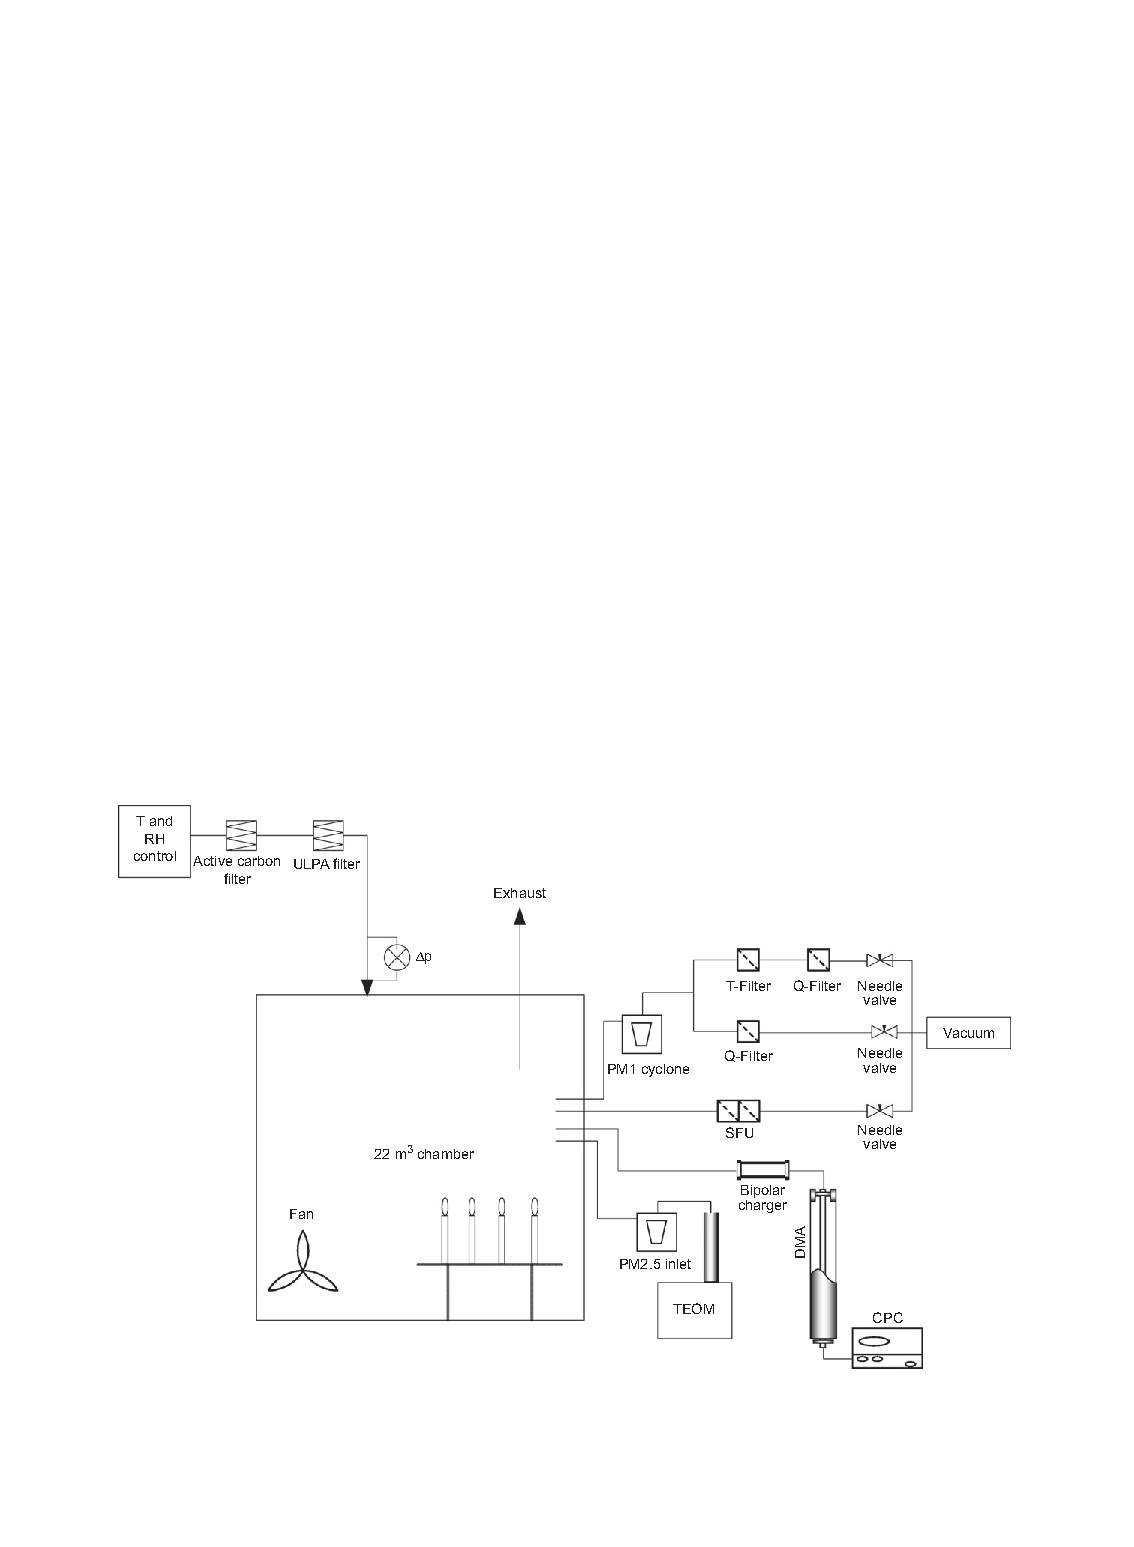
\includegraphics[width=.9\linewidth]{gfx/related/kerze_versuch.pdf}} \quad
	\caption[Versuchsaufbau zur Ermittlung der chemischen Zusammensetzung von Kerzenrauch (Quelle: \cite{kerze}, S.195)]
	{Versuchsaufbau zur Ermittlung der chemischen Zusammensetzung von Kerzenrauch (Quelle: \cite{kerze}, S.195)}
	\label{fig:kerze_exp}
\end{figure} 

Auf direkte Nachfrage hin beim Hersteller der Partikelmessger\"{a}te, wie die angegebenen Werte in den technischen Dokumentationen verifiziert wurden, wiesen diese lediglich darauf hin, dass die Partikelmessger\"{a}te mit Hilfe von Aerosolgeneratoren kalibriert werden. Dies entspricht der Standardvorgehensweise zur Kalibrierung solcher Messger\"{a}te, wie sie in den VDI Richtlinien zu finden sind. Aus diesen liesen sich Kenngr\"{o}{\ss}en und Richtlinien an die zu verwendeten Aerosolgeneratoren ableiten, welche in der Reinraumtechnik Verwendung finden.
\\\\
Uns sind letzendlich keine Versuchsaufbauten bekannt, welche ausschlie{\ss}lich zur Identifizierung der Zeitkonstante eines Partikelmessger\"{a}ts dienen. Zudem lies sich die Zeitkonstante aus keinem der uns vorliegenden Handb\"{u}cher entnehmen die darauf hindeuten w\"{u}rden, dass es ein existierendes Verfahren gibt diese zu messen. 